\documentclass{article}
\usepackage[utf8]{inputenc}
\usepackage{hyperref}
\usepackage{geometry}
\usepackage{amsmath}
\usepackage{subcaption}
\usepackage{graphicx}
\usepackage{tikz}
\usepackage{fancyhdr}
\usepackage{amssymb}
\usepackage{multicol}
\hypersetup{
    colorlinks=true,
    linkcolor=black,
    filecolor=magenta,      
    urlcolor=cyan,
    pdftitle={Overleaf Example},
    pdfpagemode=FullScreen,
    }
\title{Methoden & Technieken}
\author{Kristo Wind}
\date{September 2022}

\geometry{
 a4paper,
 total={170mm,257mm},
 left=20mm,
 top=25mm,
 bottom=20mm,
 }
\begin{document}

\begin{titlepage}
\newgeometry{left=3cm,bottom=1.5cm}
    \begin{center}
        \begin{minipage}{0.43\textwidth}
        \rule{0.9\linewidth}{0mm}\\
        \vspace{0.5cm}
        \end{minipage}
        
        
\vspace{1cm}
        \rule{\linewidth}{2pt}
        
        \vspace{0.7em} 
        {\LARGE \bfseries Methoden en Technieken: Supervised Machine Learning}
         
        
        \rule{\linewidth}{2pt} \\
        {\sc Hogeschool van Amsterdam  -  Master Applied Artificial Intelligence}\\
    \vspace{8cm}
     {\large \sc  \textit{\textbf{Kristo Wind}}}\vspace{4cm}

   

    \end{center}
    
    \vspace{3.3cm}
    \begin{figure}[htb]
        \centering
        \includegraphics[width=0.15\linewidth]{Images/logo2.png}
        \label{fig:hemoglobin3d}
    \end{figure}
    \begin{center}
        \makeatletter
        Amsterdam \\
        November 2022
        \makeatother
    \end{center}
\end{titlepage}

\newpage
\setcounter{page}{1}
\pagestyle{plain}

\pagestyle{fancy}
\fancyhf{}
\cfoot{\thepage}
\fancyhead[L]{\leftmark}
\renewcommand{\footrulewidth}{0.5pt}
\rfoot{\includegraphics[width=4cm]{Images/HVA.png}}

{\large
\begin{center}
    {\Large \textbf{Methoden en Technieken: Supervised ML}}\\
\end{center}
\tableofcontents
\newpage
\section*{Data-analyse stappenplan}
\begin{enumerate}
    \item Dataset altijd eerst ruwe data, zoals fotos of punten op assenstelsel. Eerst gevoel krijgen voor de data.
    \item Hoeveel verschillende soorten data. Mist er data? 
    \item Willekeurige plots maken.
    \item logaritme van inkomen vertalen het beter. 
    \item Afmetingen bekijken.
    \item Min-max waarden.
    \item Aantal fotos per persoon op volgorde (df.value\_counts(subset='Name')).
    \item Histogram plotten (plt.hist(counts[:,1], bins=30)).
    \item Voor balans in data, augmenteren.
\end{enumerate}
\newpage
\textbf{{\LARGE Week 1}}\\
Aandachtspunten:
\begin{itemize}
    \item Leerdoelen 7, 8, 9, 12
    \item $E(\bar{X})=\mu$ %blz. 106 LaTeX symbol list
    \item $Y=f(X)+\epsilon$
    \item Flexibiliteit van een model
    \item \href{https://hastie.su.domains/ISLR2/ISLRv2_website.pdf}{Statistical Learning hoofdstuk 2}.
    \begin{itemize}
        \item prediction \& inference (regressie)
        \item parametric \& non-parametric methods (regressie)
        \item The Bayes Classifier (classificatie)
    \end{itemize}
\end{itemize}

\section{Basiskennis statistiek en kansrekening}
\begin{center}
    $E(\bar{X})=\mu$
\end{center}
\noindent $\bar{X}$ = steekproefgemiddelde (unbiased estimator)\\
$\mu$ = populatiegemiddelde\\
$E$ = verwachtingswaarde\\ \vspace{0.3cm}

\noindent Waarom statistiek en kansrekening?
\begin{itemize}
    \item Wat is het percentage minderjarige bezoekers per dag?
    \item Is dat elke dag hetzelfde?
    \item Wat is het gemiddelde percentage minderjarige bezoekers per dag?
    \item Wat is, gemeten over een maand, het gemiddelde percentage minderjarige bezoekers per dag?
    \item Wat zegt dit over het werkelijke gemiddelde percentage minderjarige bezoekers per dag?
    \item Wat zegt dit over het werkelijke percentage minderjarige bezoekers op een dag?
\end{itemize}\vspace{0.5cm}


\textbf{Voorbeeld ML-vraagstuk} (regressie)\\
\noindent Het bepalen van de leeftijd van de klant adhv de variabele gewicht komt wiskundig neer op het bepalen van de $f$ in de volgende vergelijking:\\
\begin{center}
    $Y=f(X)+\epsilon$\\
\end{center}

\noindent
Met $Y$ de leeftijd van de klant, $X$ het gewicht van de klant en $\epsilon$ de fout-term.\\
$f$: de informatie in $X$ over $Y$ (deterministisch: temaken met een kans)\\
$\epsilon$: dat wat we niet kunnen weten over Y, gegeven X (stochastisch). Het verschil voorspelde leeftijd en echte leeftijd\\

\noindent Leren: het schatten van functie $f$. Data gebruiken is essentieel. Als we $f$ op een andere manier zouden bepalen (bijv. uit theoretische overwegingen) zal het niet leren worden genoemd.\\

\noindent Diverse ontwerpkeuzes die behandelt dienen te worden. Onderstaande bepaald adhv de opdracht en is de ontwerpvraag.\\
\begin{itemize}
    \item Classificatie of regressie?
    \item Welke foutmaat? Wat wil je minimaliseren?
    \item Voorspellen of samenhang? Blackbox al goed of wil je weten hoe?
\end{itemize}\vspace{0.3cm}
\noindent Onderstaand wordt het model genoemd (hypothesis set en algoritme samen)
\begin{itemize}
    \item Welke functies om $f$ te schatten (hypothesis set)?
    \item Welk algoritme om de beste $\hat{f}$ te vinden?
\end{itemize}\vspace{0.5cm}


\section{Flexibiliteit van het model (om f proberen te schatten)} 
\noindent Kans is aanwezig dat $f$ niet lineair van $X$ afhangt en dat de foutmaat kleiner wordt als we een flexibeler model kiezen (hypotheseruimte groter maken). Hoe meer termen, hoe meer kans op overfitting. $\hat{f}(X)=\hat{\beta_0}+\hat{\beta_1}X$ is lineair bijvoorbeeld. De onderstaande polynoom niet.\\
\begin{center}
$\hat{f}X)=\hat{\beta_0}+\hat{\beta_1}X+\hat{\beta_2}X^2+\hat{\beta_3}X^3+\hat{\beta_4}X^4$
\end{center}

\subsection{De bias-variance tradeoff}
\begin{figure}[h]
    \centering
    \includegraphics[width=0.4\linewidth]{Images/biasvariance.png}
    \caption{bias-variance}
    \label{fig:biasvariance}
\end{figure}
Als data wordt weergegeven door:
\begin{center}
    $(x_1,y_1),(x_2,y_2),..,(x_n,y_n)$
\end{center}
dan wordt de foutmaat gegeven door de mean squared error (MSE):
\begin{center}
    $MSE=E[(Y-\hat{f}(x_0))^2]=Var(\hat{f}(x_0))+(f(x_0)-E[\hat{f}(x_0))^2+Var(\epsilon)=Var(\hat{f}(x_0))+B(\hat{f}(x_0))^2+Var(\epsilon)$
\end{center}
\noindent Waarbij:\\
1e term: de spreiding van de steekproef (hoe groot is het wolkje?) \\
2e term: als 0 = geen gemiddelde afwijking = geen bias (hoeveel zit je gemiddeld af van de roos ($\mu$)\\
3e term: de spreiding van de error-term\\
Met aannames:
\begin{enumerate}
    \item $Var(X)=E(X^2)-E(X)^2$
    \item $E(\epsilon)=0$
    \item $Cov(X,\epsilon)=0$
\end{enumerate}


\section{Statistical Learning} \vspace{1mm}\\
\noindent \textbf{inputs} ($X_1, X_2,..., X_p$) = predictors, independent variables, features, variables\\
\textbf{output}($Y$) = response, dependent variable\\

\noindent \textbf{Prediction}: When function $f$ is not neccessary to determine (blackbox).
\begin{itemize}
    \item \textit{predict the response using predictors.}
\end{itemize}\vspace{3mm}


\noindent \textbf{Inference}: Need to know function $f$.
\begin{itemize}
    \item \textit{Which media are associated with sales?}
    \item \textit{Which media generate the biggest boost in sales?}
    \item \textit{To what extent is the product's price associated with sales?}
\end{itemize}\vspace{3mm}

\textbf{Estimate $f$:}
\begin{itemize}
    \item Parametric methods
    \item Non-parametric methods
\end{itemize}\vspace{3mm}

\textbf{\textit{Parametric methods (inflexible)}}:
\begin{enumerate}
    \item Make an assumption about the functional form of shape of $f$ (linear).
    \item Need an approach to fit the model.
\end{enumerate}
Answers:
\begin{enumerate}
    \item $Y\approx\beta_0+\beta_1X_1+\beta_2X_2+...+\beta_pX_p$.
    \item (ordinary) least squares is most common.
\end{enumerate}

\subsection{Non-parametrische methoden (flexibel)}
Non-parametric methods do not make explicit assumptions about the functional form of $f$. Instead they seek an estimate of $f$ that gets as close to the data point as possible without being too rough of wiggly.
\begin{figure}[h!]
    \centering
    \begin{subfigure}{0.3\textwidth}
        \centering
        \includegraphics[width=\linewidth]{Images/lineaire regressie plot.png}
        \caption{Linear (parametric)}
        \label{fig:parametric}
    \end{subfigure}
    \:
    \begin{subfigure}{0.3\textwidth}
        \centering
        \includegraphics[width=\linewidth]{Images/flexibele regressie.png}
        \caption{Flexible (non-parametric)}
        \label{fig:non-parametric}
    \end{subfigure}
    \:
    \begin{subfigure}{0.3\textwidth}
        \centering
        \includegraphics[width=\linewidth]{Images/overfitting.png}
        \caption{Too flexible (overfitting)}
        \label{fig:overfitting}
    \end{subfigure}
    \caption*{}\vspace{-3mm}
    \label{fig:3dplots}
\end{figure}

\noindent Regressie: kwantitatief\\
Classificatie: kwalitatief\\

\noindent Cross-validatie (zie week 4): estimation method for estimating test MSE using the training data (MSE = optimal combination of bias \& variance).\\
Good performance: low squared bias \& low variance.

\section{Classificatie}
\begin{itemize}
    \item The Bayes Classifier
    \item KNN
\end{itemize}

\subsection{The Bayes Classifier}
The line where $Pr(Y=j|X=x_0)$ is exactly 0.5, with error $1-E(\max\limits_{j}Pr(Y=j|X))$.
\begin{figure}[h]
    \centering
    \includegraphics[width=0.5\linewidth]{Images/bayes method.png}
    \caption{Bayes Classifier}
    \label{fig:knn}
\end{figure}
}

\newpage
{\large
\textbf{{\LARGE Week 2}}\\
Aandachtspunten:
\begin{itemize}
    \item KNN (classificatie)
    \item \href{https://work.caltech.edu/telecourse}{Learning from Data}
    \item Regularisatie ($l_1$ en  $l_2$)
\end{itemize}
\subsection{K-Nearest Neighbors (KNN)}
The line where $Pr(Y=j|X=x_0)=\frac{1}{K}\sum\limits_{i\in\mathcal{N}_0}I(y_i=j)$.\\
$\mathcal{N}_0$ represents the training data closest to $x_0$.\\

\begin{figure}[h]
    \centering
    \includegraphics[width=0.8\linewidth]{Images/KNNmodels.png}
    \caption{K-Nearest Neighbors algorithm}
    \label{fig:knn}
\end{figure}

\[\textrm{expected test-MSE} = E[Y-g(x_0))^2]=Var(Y)+(E(Y)-g(x_0))^2=Var(\epsilon)+(f(x_0)-g(x_0))^2\].
\[Var(X)=E(X^2)-E(X)^2\]
\[E(X^2)=Var(X)+E(X)^2\]
\[E((Y-g(x_0))^2)=Var(Y-g(x_0))+E(Y-g(x_0))^2=\]
\[=Var(Y)+(E(Y)-g(x_0))^2=Var(\epsilon)+(E(Y)-g(x_0))^2\].\vspace{2mm}
Waarbij $g^*(x_0)$ is het minimum en wordt gegeven door $g^*(x_0)=f(x_0)=E(Y|X=x_0)$.\vspace{2mm}\\
$Var(g(x_0))$ is 0, want is een vaste waarde en $E(g(x_0))=g(x_0)$ want verwachtingswaarde van vaste waarde is de vaste waarde.\\
$g(x_0)=E(Y|X=x_0)$ geeft bijvoorbeeld voor iemand van 80kg een gemiddelde van de $k$ mensen die het dicht bij de 80kg liggen, dus KNN benadering.

\subsection{Foutmaten}
Regressie:
\begin{itemize}
    \item MSE (mean squared error)
    \item MAE (mean absolute error): de optimale $f(X)$ gegeven worden door de voorwaardelijke mediaan van Y gegeven X. 
\end{itemize}
\noindent Classificatie:
\begin{itemize}
    \item Accuracy
    \item Bayes classifier
\end{itemize}
\subsubsection{Accuracy}
Train error rate$=\frac{1}{n}\sum\limits_{i=1}^nI(y_i\neq\hat{y}_i)$
met:
\[I(y_i\neq\hat{y}_i)=\begin{cases}
    1, & \text{if }\hspace{2mm} y_i\neq\hat{y}_i\\
    0, & \text{if}\hspace{3mm} y_i=\hat{y}_i
\end{cases}\]

\subsubsection{Bayes classifier}
De functie $f^*(x_0)$ met laagste test error rate is de Bayes classifier gegeven door:
$f^*(x_0)=C_j$ met $P(Y=C_j|X=x_0)=max_i(P(Y=C_i|X=x_0))$. De klasse $C_i$ met de hoogste kans ($max_i(P(Y=C_i|X=x_0))$) als $x_0$ gegeven, wordt klasse $C_j$ de uitkomst van de optimale functie $f^*(x_0)$.\\

\subsection{Verschil lineaire regressie en KNN-regressie}
\noindent $f(x)=E(y|x)$ is lineaire regressie aanname. KNN probeert $E(y|x)$ zonder aannames te schatten door omringende waarden te analyseren. Stel data hangt lineair samen, kan je $f(x)=E(y|x)$ wel aannemen. Meer datapunten nodig voor KNN tov van lineaire regressie om zekerder te zijn dat er minder fouten op de testdata voorkomen. Het aantal waarnemingen dat je nodig hebt, hoe groter de functieruimte is. Minder waarnemingen, minder flexibel model. Overweging tussen lineaire regressie en KNN hangt af van overfitting. KNN heeft mogelijkheid tot overfitting waar lineaire regressie dat niet heeft.\\

\section{Lineaire regressie}
\[Y=\beta_0+\beta_1X_1+\beta_2X_2+...+\beta_pX_p+\epsilon\]
Lineaire regressie slaat niet op de macht van $X$, maar op de $\beta$. Want $X$ en $Y$ zijn gegeven. In termen van de coëfficiënten is de vergelijking lineair. Dus onderstaande vergelijking is ook lineair:
\[Y=\beta_0+\beta_1X_1+\epsilon\]
\noindent Eigenschappen van $\hat{\beta}_j$:
\begin{itemize}
    \item schatters $\hat{\beta}_j$ zijn zuiver: $E(\hat{\beta}_j)=\beta_j$
    \item de verdeling van de schatters is bekend
\end{itemize}
95\% betrouwbaarheidsinterval: als je oneindig keer steekproef doet valt $\hat{Y}$ in 95\% van de gevallen in $Y$.\\
\begin{multicols}{2}

\noindent Voordelen lineaire regressie:
\begin{itemize}
    \item Hoge interpreteerbaarheid
    \item Bij beperkt aantal waarnemingen goed bruikbaar
    \item Grote storingen goed bruikbaar
    \item Bij sparse data goed bruikbaar
    \item Door gebruik te maken van transformaties toch redelijk flexibel
\end{itemize}


\noindent Wat kan er misgaan?
\begin{itemize}
    \item $Y$ hangt niet lineair van $X_1, X_2,...,X_p$ af
    \item Correlatie tussen storingstermen
    \item Niet-constante variantie van de storingen
    \item Uitschieters
    \item Punten met veel invloed
    \item Collineaire variabelen
   % \item te weinig waarnemingen
\end{itemize}
\end{multicols}
\noindent Vuistregel Robert: 'Aantal parameters mag niet zelfde orde van grote hebben als het aantal waarnemingen. Ten minste 10x zo veel waarnemingen voor een goede voorspelling. Als die waarnemingen niet aanwezig zijn kan ridge-regressie gebruikt worden om een goede voorspelling (i.e. variantie verlagen) te genereren.'

\section{Regularisatie}
\subsection{Ridge-regressie}
Laat de $n$ waarnemingen van de train-data gegeven zijn door
\[(x_{i1},x_{i2},...,x_{ip},y_i), \textrm{ met } i \in {1,2...,n}\]
Dan wordt de foutmaat in ridge-regressie gegeven door 
\[\textrm{ridge-fout}=\sum\limits_{i=1}^n(y_i-\beta_0-\sum\limits_{j=1}^p\beta_jX_{ij})^2+\lambda\sum\limits_{j=1}^p\beta_j^2\]
met $\lambda$ een waarde die de tuning-parameter wordt genoemd. Bij kleine $\lambda$ mag beta-schijf groter en bij grote $\lambda$ ben je streng en mag beta-schijf niet groter. Ridge-regressie maakt gebruik van $l_2$-regularisatie ($\beta_1^2+\beta_2^2<1$).Kleinere coëfficiënten impliceert eenvoudigere functies om overfitting tegen te gaan. Door middel van \textbf{cross-validatie} kan je de $\lambda$ bepalen. Een juiste $\lambda$ zal ervoor kunnen zorgen dat de variantie meer daalt dan de onzuiverheid toeneemt, waardoor de test-MSE kleiner wordt.\\

\subsection{Lasso-regressie}
Lasso: least absolute shrinkage and selection operator
\[\textrm{lasso-fout}=\sum\limits_{i=1}^n(y_i-\beta_0-\sum\limits_{j=1}^p\beta_jX_{ij})^2+\lambda\sum\limits_{j=1}^p|\beta_j|\]
In plaats van de $l_2$-penalty van ridge-regressie, maakt lasso-regressie gebruik van de $l_1$-penalty ($|\beta_1|+|\beta_2|<2$). $\beta_0$ bestraf je niet en zit dus niet in de fouten.

\begin{figure}[h]
    \centering
    \includegraphics[width=0.8\linewidth]{Images/regularization.jpg}
    \caption{$l_2$-regularisatie (links) en $l_1$-regularisatie (rechts)}
    \label{fig:regularisatie}
\end{figure}

\noindent Kleine $\lambda$: kleinste kwadraten methode\\
Grote $\lambda$: niet ver zoeken, dicht bij oorsprong blijven\\
Gebruik CV om om $\lambda$ te zoeken om de ruimte te bepalen.
}

\newpage
\
\newpage
{\large
\textbf{{\LARGE Week 3}}\\
Aandachtspunten:
\begin{itemize}
    \item classificatie: foutmaat voor een kansmodel
    \item Maximum likelihood estimator (MLE)
    \item Lineaire discriminantanalyse (LDA) en principal component analyse (PCA)
\end{itemize}
\section{Classificatie: foutmaat voor een kansmodel}
informatie-entropy (loss functie):
\[\textrm{logistic loss}=-\sum\limits_{i=1}^n(y_i)ln(\hat{y_i})+(1-Y_i)ln(1-\hat{y_i})\]
\[(y_i)ln(\hat{y_i})+(1-Y_i)ln(1-\hat{y_i})=\begin{cases}
    ln(1-\hat{y_i}), & \text{if }\hspace{2mm} y_i=0\\
    ln\hat{y_i}, & \text{if}\hspace{3mm} y_i=1
\end{cases}\]
Logistische regressie:
\[ln(\frac{\hat{y}}{1-\hat{y}})=\hat{\beta}_0+\hat{\beta}_1x\]
sigmoid-activatiefunctie (i.e. sigma-transformatie) differentieert makkelijk. SGD afname is makkelijk te berekenen:
\[\frac{e^x}{1+e^x}=\sigma(x)\]
\[\sigma'(x)=\sigma(x)(1-\sigma(x))\]
Least squared gebruiken we niet, omdat gemiddelde gekwadrateerde fout geen realistische schatters geven. Willen foutmaat kiezen zodat we schatters krijgen die zich netjes gedragen en met het probleem te maken hebben. Voor regressie is LS wel goede schatter.\\

% data\xrightarrow{schatting \hat{\beta}_0, \hat{\beta}_1}\xrightarrow{kans dat je data ziet} \textrm{kans dat je data ziet}\xrightarrow{vind \hat{\beta}_0, \hat{\beta}_1 zodat kans maximaal is}

\section{Maximum likelihood estimator}
\noindent Maximum likelihood bij logistische regressie:
\[P(Y|X=x)=P(Y=1|X=x)^Y(1-P(Y=1|X=x))^{1-Y}\]
MVUE: Minimale variantie voor zuivere schatter

\noindent Logistische regressie is een uitbreiding van sigmoid met meerdere voorspellende variabelen:\\
\[\hat{y}(x_1,x_2,...,x_p)=\frac{e^{\hat{\beta}_0+\sum\limits_{i=1}^p\hat{\beta}_ix_i}}{1+e^{\hat{\beta}_0+\sum\limits_{i=1}^p\hat{\beta}_ix_i}}\]

\noindent Logistische regressie voor meer klassen (softmax):\\
\[ln(\frac{P(Y=C_1|X=x)}{P(Y=C_k|X=x)})=\beta_{10}+\beta_1x\]
\[ln(\frac{P(Y=C_2|X=x)}{P(Y=C_k|X=x)})=\beta_{20}+\beta_2x\]

\section{LDA}
In de situatie dat Y uit meer klasses $K > 2$ bestaat en dat er
meer ($p > 1$) voorspellende variabelen zijn, maken we een
vergelijkbare aanname. Namelijk dat, gegeven de klasse k voor
Y, de voorspellende variabelen een \textbf{multivariate normale
verdeling} volgen met een covariantiematrix die onafhankelijk
is van de klasse k.\\
Ook nu zal de klasse bepaald worden door
discriminantfuncties die lineair zijn in de p voorspellende
variabelen.\\

\noindent LDA met $p=1$:\\
Stel dat Y een lineaire variabele is die we willen schatten middels een continue X. Neem aan dat voor gegeven klasse $k \in {0, 1} \textrm{ van } Y$,
\[X \sim N(\mu_k,\sigma^2)\]
Als we P(Y) weten, kunnen we via de stelling van Bayes P(Y|X) uitrekenen.\\

\noindent Als men aanneemt dat de covariantiematrix van de verdeling van de voorspellende variabelen voor elke klasse k van Y verschillend mag zijn, dan worden de discriminantfuncties kwadratisch (quadratic discriminant analysis).\\
LDA is dus een speciaal geval van QDA.\\
QDA ten opzichte van LDA heeft voordelen (het is immers algemener) en nadelen (het is immers algemener).\\

\noindent Er ontstaat een kwadratisch probleem als variantie van twee klassen dermate verschilt (zie foto). Als nog meer variabelen worden toegevoegd, welke mogelijk gecorreleerd zijn (diagonaalmatrix naar $\frac{1}{Cov(X_1,X_2)}$ etc. op de plekken van de 0), functieruimte wordt veel groter (grotere vrijheidsgraden). Model flexibeler maken? Dus PCA gebruiken (demensiereductie en haalt correlaties weg tussen data).\\

\section{PCA}
$PC_1$ sla je dicht op de langste richting, op hoek van 90 graden maak je $PC_2$ (matrix diagonaliseren, programma vind een rotatie). Zodoende vallen de correlaties weg. \\

\begin{figure}[h]
    \centering
    \includegraphics[width=0.6\linewidth]{Images/pca.png}
    \caption{Principal component analysis}
    \label{fig:pca}
\end{figure}
\noindent $PC_1$ beschikt over 90\% van de variantie, dus andere PCAs zijn ruis. 

\noindent Foto’s zijn eigenlijk zeer hoog dimensionale waarnemingen. Een PCA uitgevoerd op een dataset van foto's van gezichten word ook wel Eigenfaces genoemd.\\
\begin{figure}[h]
    \centering
    \includegraphics[width=0.8\linewidth]{Images/pca1.png}
    \caption{PCA's van gezichten}
    \label{fig:pca1}
\end{figure}

\noindent Het idee is dat iedere foto geschreven kan worden als een lineaire combinatie van Eigenfaces:
\begin{figure}[h]
    \centering
    \includegraphics[width=0.8\linewidth]{Images/pc2.png}
    \caption{PCA samenhang op een gezicht}
    \label{fig:pca2}
\end{figure}

\subsection{PCR}
Principal components regression (PCR) of hoofdcomponenten-regressie bestaat uit een regressie-analyse op de eerste M hoofdcomponenten. De aanname van PCR is dat de richtingen waarin de voorspellende variabelen het meest variëren ook de richting zijn die het meest de variatie van Y kunnen verklaren.\\

\noindent Eerst PCA uitvoeren (als correlatie), een aantal PC's waar je regressieanalyse op uitvoert. Dus niet regressie op $X_1$ en $X_2$, maar op $PC_1$ en $PC_2$.\\

}

\newpage
{\large
\textbf{{\LARGE Week 4}}\\
Aandachtspunten:
\begin{itemize}
    \item Modelbeoordeling en -selectie: Resampling methods
    \item Data snooping, data leakage (\href{https://arxiv.org/pdf/2207.07048.pdf}{Leakage and the Reproducibility Crisis in ML-based Science})
    \begin{itemize}
        \item zie taxonomy template in Data\_leakage\_taxonomy.docx in ../Vakken/MenT
    \end{itemize}
\end{itemize}
\section{Resampling methods}
Manieren om iets te kunnen zeggen over de variantie van de schatting. Onderstaande methoden worden gebruikt om een \textbf{model te beoordelen} op testdata en het \textbf{selecteren van een model} (welk niveau van flexibiliteit):
\begin{enumerate}
    \item Cross-validatie
    \item Bootstrap
\end{enumerate}
\subsection{Cross-validatie}
Train-test split kan ook gesplitst worden in train-val-test split (train set nog een keer splitsen). Train met verschillende waarden voor hyperparameters op de trainset en beoordeel de prestatie van de modellen op de validatieset. Nadelen zijn dat de fout-maat op de validatie afhankelijk is van de splitsing en je hebt een kleinere trainset waardoor de schatting van de fout-maat minder goed is (mogelijk een bias). Oplossing is \textbf{Leave-one-out cross-validation (LOOCV)}:

\subsubsection{LOOVC}
\noindent Trainset van $n$ waarnemingen. Splits de trainset $n$ keer in een:
\begin{itemize}
    \item nieuwe trainset van $n-1$ waarnemingen, en
    \item een validatieset van overgebleven waarneming
\end{itemize}
Met als fout-maat de gemiddelde foutmaat op de $n$ verschillende validatiesets. Zodoende wordt de trainset nauwelijks kleiner en is de foutmaat niet afhankelijk van de splitsing.\\

\subsubsection{$k$-fold CV}
Moet $n$ keer getraind worden op $n-1$ waarnemingen. Dus, \textbf{$k$-fold cross-validation ($k$-fold CV)} gebruiken:\\
Stel dat we de hyperparameter $\lambda$ willen tunen (bijvoorbeeld KNN om $k$ te tunen):
\begin{itemize}
    \item Definieer $M$ verschillende waarden $\lambda_1, \lambda_2,..., \lambda_M$ voor $\lambda$
    \item Bepaald voor elke waarde $m \in {1,...,M}$ middels $k$-fold CV de gemiddelde foutmaat $E_{CV}(m)$
    \item kies die waarde $m^*$ voor $m$ waarvoor $E_{CV}(m)$ het laagst is
    \item train opnieuw, maar nu op de gehele dataset en $\lambda_{m^*}$
\end{itemize}
Vuistregel: gebruik k=10 en gebruik honderd waarnemingen om slechts enkele parameters te tunen.\\

\noindent Wat kan $\lambda$ zijn?:
\begin{itemize}
    \item Wat is het type model dat wil ik gebruiken?
    \begin{itemize}
        \item lineair of NN of SVM
        \item polynomiaal model: tot hoeveelste orde
        \item keuze voor tuning-parameter in regularisatie
    \end{itemize}
\end{itemize}

\subsection{Bootstrapping} (doen alsof er meer data is om achter de variantie van je steekproefgemiddelde te komen.)\\
Is een manier om de variantie van een schatter te schatten middels steekproeven uit een steekproef:
\begin{itemize}
    \item oorspronkelijke steekproef $S$ van $n$ waarnemingen
    \item Trek met teruglegging $B$ steekproeven van $n$ waarnemingen
    \item Laat $\hat{\alpha}$ geschat zijn met $S$
    \item Het idee van bootstrapping is dat we de verdeling van $\hat{\alpha}$ kunnen schatten middels de geschatte parameters $\hat{\alpha}^{*b}$ $(b \in {1, 2,.., B})$ die geschat zijn op de B steekproeven.
    \item Een schatting voor de variantie van ˆα zal gegeven worden
door de steekproefvariantie van de $\hat{\alpha}^{*b}$
\end{itemize}
Waarom zou je bootstrapping willen toepassen?:\\
Als de variantie heel hoog is, is de zekerheid laag. Je wilt met bepaalde zekerheid zeggen dat het steekproefgemiddelde een bepaalde waarde heeft.

\noindent Hyperparameter: parameters om leerproces aan te sturen\\
Parameter: gewichten/coëfficiënten = uitkomsten na leren\\

\subsection{Data snooping/data leakage}
\begin{itemize}
    \item Geen correcte train-test-splitsing
    \begin{itemize}
        \item Geen testset
        \item Datapreparatie op train- en testset
        \item Variabelenselectie op train- en testset
        \item Dubbelingen in testset
    \end{itemize}
    \item Verkeerde variabelen
    \begin{itemize}
        \item Medicijngebruik om hoge bloeddruk te meten
    \end{itemize}
    \item Testset is niet representatief
    \begin{itemize}
        \item Lekkage in de tijd (om een voorspelling in de tijd te maken, hoort de train-set voor de testset hebben plaatsgevonden)
        \item Geen oafhankelijkheid tussen train- en testset (voorbeeld: verschillende waarnemingen van dezelfde persoon in de train- en testset)
        \item Bias in testset
        \begin{itemize}
            \item Testset van specifieke regio, maar iets beweren over alle regio's
            \item Ongewenste waarnemingen weglaten uit de testset
        \end{itemize}
    \end{itemize}
\end{itemize}
}

\newpage
{\large
\textbf{{\LARGE Week 5}}\\
Aandachtspunten:
\begin{itemize}
    \item Beslisbomen regressie
    \item Beslisbomen classificatie
    \item Ensemble-technieken
\end{itemize}

\section{Beslisbomen regressie}\\
De foutmaat voor regressie met een beslisboom zal dan
gegeven worden door
\[RSS=\sum\limits_{j-1}^J\sum\limits_{i\in R_j}(y_i-\hat{y}_{R_j})^2\]
Het doel van een beslisboom voor regressie zal zijn de J niet
overlappende regio’s $R_1, R_2,... , R_J$ te vinden zo dat RSS
geminimaliseerd wordt.

\subsection{Het algoritme}
\begin{enumerate}
    \item Kies de variabele $X_j$ en de waarde $s$ zo dat de regio's 
    \[\{X|X_j<s\} \textrm{ en } \{X|X_j\geq s\}\]
    de RSS minimaliseren.
    \item Kies één van bovenstaande regio’s en herhaal
bovenstaande stap. De regio, variabele en waarde wordt
zo gekozen dat het de RSS minimaliseert.
    \item Herhaal bovenstaande stap tot een stop-criterium wordt
bereikt. Bijvoorbeeld: geen enkele regio heeft meer dan
vijf trainpunten.
\end{enumerate}

\subsubsection{Keuze voor algoritme}\\
\noindent Dit algoritme zorgt voor rechthoekige gebieden.\\

\noindent Dit is een voorbeeld van een \textit{greedy} algoritme. (greedy algoritme kijkt maar 1 stap vooruit, dat hoeft niet beter te zijn. Om op te lossen: pruning/snoeien)\\

\noindent De bomen die hier uit volgen kunnen behoorlijk complex zijn
(erg veel gebieden).\\

\noindent We zouden als stop-criterium kunnen gebruiken dat elke stap
de RSS met minstens een bepaalde waarde verlaagd. Een
nadeel van deze methode is dat dit weer te rigide is. Er zou
een zeer goede stap, na een vrij slechte stap kunnen komen.\\

Om overfitting tegen te gaan, kunnen we een deelboom van
de oorspronkelijke boom gebruiken (snoeien, pruning).\\

\noindent We zouden die deelboom willen kiezen die de test-RSS
minimaliseert. Cross-validation op alle deelbomen is niet altijd
mogelijk.\\

\noindent Gebruik om te snoeien de volgende fout-maat
\[\textrm{cost-complexity-maat}=\sum\limits_{m=1}^{|T|}\sum\limits_{x_i\in R_m}(y_i-\hat{y}_{R_m})^2+\alpha|T|\]
waar $|T|$ staat voor het aantal eindpunten van de boom $T$.\\

\subsection{Cost complexity pruning (weakest link pruning)}
\begin{enumerate}
    \item Recursive binary splitting met stopcriterium op de traindata: volledige boom
    \item Cost complexity pruning op de boom uit de vorige stap: rij van deelbomen afhankelijk van $\alpha$
    \item $\alpha$ bepaald je met cross-validatie met gemiddelde RSS. Voor elke $k \in \{1,2,..,.K\}$
    \begin{enumerate}
        \item Herhaal stap 1 en 2 op de nieuwe traindata
        \item Bepaal de RSS op de validatieset als functie van $\alpha$
    \end{enumerate}
    De deelboom uit 2 met $\alpha$ uit 3
\end{enumerate}

\section{Beslisbomen classificatie}\\
Ook nu verdelen we de ruimte van voorspellende variabelen in $J$ niet overlappende regio's $R_1,R_2,...,R_J$.\\

\noindent Stel dat een datapunt ($x_1,x_2,...,x_p$) in regio $R_j$ valt, dan zal de voorspelling bij een beslisboom voor classificatie gegeven worden door:
\[\hat{y}(x_1,x_2,...,x_p)=\hat{y}_{R_j}\]
waar $\hat{y}_{R_j}$ staat voor de klasse waar de meeste $y_i\in R_j$ vallen.\\

\noindent De foutmaten voor een classificatie beslisboom worden gegeven door twee maten. Het is gebruikelijk om de Gini-index of de entropie te gebruiken om de ruimte te splitsen. Dit zal zorgen voor regio’s met hoge en lage fracties:
\[\textrm{Gini index}= \sum\limits_{k=1}^K\hat{p}_{mk}(1-\hat{p}_{mk})\]
\[\textrm{entropy}=\sum\limits_{k=1}^K\hat{p}_{mk}log(\hat{p}_{mk})\]
waarbij $\hat{p}_{mk}$ de fractie van traindata in regio $R_m$ van klasse $k$ zijn.\\

\noindent Daarnaast is het gebruikelijk om de error-rate te gebruiken als de accuraatheid van belang is voor het snoeien van de boom:
\[\textrm{error-rate}=1-max\limits_{k}(\hat{p}_{mk})\]

\section{Ensemble-technieken}\\
Beslisbomen hebben een hoge variantie, door traindata aan te passen ontstaat meteen een hele andere boom. Bij ensemble methoden neem je het gemiddelde van uitkomsten van meerdere simpele modellen.\\
\[Var(x)=\sigma^2 \rightarrow Var(\Bar{x})=\frac{\sigma^2}{n}\]
Des te hoger $n$, des te lager je variantie. Door ieder model een andere steekproef te geven verhoog je n en zo verlaag je de variantie.\\

\noindent Moet je zorgen dat de modellen onafhankelijk zijn $\rightarrow$ ieder model eigen steekproef. Anders dan $k$-fold omdat je modellen daar niet onafhankelijk zijn.\\

\noindent De simpele modellen die je middelt noem je 'weak learners'. Die hebben misschien een hoge bias, maar die middel je weg.
\begin{itemize}
    \item weak learner is iets beter dan een naïef-nul-model
    \begin{itemize}
        \item die voorspelt altijd gemiddeld $y$ of random gok bij binaire classificatie.
    \end{itemize}
\end{itemize}

\subsection{Bagging (regressie)}
\begin{itemize}
    \item Bootstrap aggregation
    \begin{itemize}
        \item Bij bootstrap pak je $B$ voorbeelden zonder terugleggen, zo maak je steekproeven en zeg je iets over de variantie.
    \end{itemize}
    \item Bagging
    \begin{itemize}
        \item trek B steekproeven en zoek voor elke $k \in B$ een model
    \end{itemize}
\end{itemize}
Laat $f^{*b}(x)$ het model zijn uit steekproef b, dan geldt voor regressie:
\[\hat{f}_{bag}(x)=\frac{1}{B}\sum\limits_{i-1}^Bf^{*b}(x)\]
Voor classificatie geldt: meeste stemmen gelden.\\

\noindent Een waarneming die niet in de steekproef $b$ zit noemen we out-of-bag. Deze data gebruik je om te testen. Dus om f(2) OOB te testen, gebruik ik 1 en 3, want voor hun is 2 de geschikte testdata.\\
\begin{table}[h]
    \centering
    \begin{tabular}{c|c|c}
         b & b \{1,2,3\} & OOB \\ \hline
         1 & 1, 1, 1 & 2, 3\\
         2 & 3, 2, 3 & 1\\
         3 & 1, 3, 3 & 2 \\
    \end{tabular}
    \caption*{}
    \label{tab:my_label}
\end{table}
\noindent
Als $b$ groot genoeg is, is de OOB-fout gelijk aan de LOOCV-fout. Bagging is nauwkeuriger maar minder interpreteerbaar.\\

\subsection{Random forest}
\noindent Random forest wordt gemaakt uit bagged bomen, waarbij elke boom een gelimiteerd aantal features heeft met $m<p$. Bij random forest is het error landschap onbekend, je zoekt naar een minimum, maar de kans is groot dat je een lokaal minimum vindt. Als er een sterke voorspeller is $q\in p$ dan begint elke boom het zelfde en is er correlatie in modellen. Want een boom is greedy. Zo blijf je hangen in het lokale minimum. Door andere variabelen de-correleer je. $m$ is de tuning parameter. Je geeft zo flexibiliteit om van A naar B te hupsen (waarbij A een lokaal minimum is en B het echte minimum).\\

\noindent $m$ bepaal je met OOB-error (out-of-bag). De OOB-voorspelling zal een goede maat kunnen zijn voor een test-voorspelling. De OOB-error is de foutmaat volgend uit de OOB-voorspellingen en is een geldige schatting van de test-error op het bagged model. Als $B$ groot genoeg is, is de ))B-error equivalent met de LOOCV-fout. Er zijn vuistregels en deze zijn zelf te tunen. Bij sterk gecorreleerde waarden moet $m$ klein zijn.\\
\begin{itemize}
    \item Regressie: $m=\lfloor \sqrt{p}\rfloor$ 
    \item Classificatie:  $m=\lfloor \frac{p}{3}\rfloor$ 
\end{itemize}
Hoe groot moet $B$ zijn in bagging?\\
Een hogere $B$ zorgt niet voor overfitting, maar kost alleen tijd. Plot ))B-error en kies $B$ waar die stabiliseert. Standaard is 100 of 500. Random forests worden niet gebruikt voor computer vision.\\

\subsection{Boosting}
\subsubsection{Het idee:}
\begin{enumerate}
    \item we gebruiken eenvoudige modellen (beslisboom met $d$ beslissingen).
    \item We fitten een ander model op storingen van het vorige model.
    \item Het nieuwe model wordt dan het vorige model plus het andere model (maal $\lambda$).
    \item Dit doen we $B$ keer en we middelen over alle uiteindelijke $B$ modellen.
\end{enumerate}

\subsubsection{Het algoritme}
\begin{enumerate}
    \item Laat $\hat{f}(x)=0$ en $r_i=y_i$ voor alle $x_i$ in trainset
    \item Voor $b \in \{1,2,...,B\}$ herhaal
    \begin{enumerate}
        \item Fit een boom $\hat{f}^b$ met $d$ beslissingen op de trainset $(X,r)$
        \item Update de voorspelling:
        \[\hat{f}(x) \leftarrow \hat{f}(x)+ \lambda\hat{f}^b(x) \]
        \item Update de storing:
        \[r_i \leftarrow r_i-\lambda\hat{f}^b(x_i)\]
    \end{enumerate}
    \item Boosted model:
    \[\hat{f}(x)=\sum\limits_{b=1}^B\lambda\hat{f}^b(x)\]
\end{enumerate}

\subsubsection{De tuning parameters}
\begin{enumerate}
    \item Het aantal bomen $B$. Boosting kan overfitten als $B$ te groot is: cross-validation.
    \item Shrinkage parameter $\lambda$ (klein en positief). Vuistregel: 0,01 of 0,001.
    \item Het aantal beslissingen $d$. Dit bepaalt de complexiteit. Meestal $d=1$, een $d$ van ongeveer 5 werkt meestal even goed als $d$ uit cross-validation
\end{enumerate}

\subsection{Bayesian Additive Regression Tree (BART)}\\
\noindent Een BART-model maakt gebruik van een bagging (middelen over bomen die op andere steekproeven dan de dataset gefit) en boosting (middelen bomen die fitten op de fout van vorige boom) idee:
\begin{itemize}
    \item Elke boom is willekeurig
    \item Elke boom bouwt op de storing van de vorige 
\end{itemize}

\subsubsection{Het idee}
\begin{enumerate}
    \item Zodra we voor gegeven iteratie $b$ en gegeven boom $k$ de partiële storing hebben berekend, fitten we een nieuwe boom ($\hat{f}_k^b$) op de data ($X,r)$.
    \item We eisen dat de nieuwe boom een perturbatie (nieuwe takken snoeien en uitkomst wijzigen) van de oude boom uit de vorige iteratie zal zijn.
\end{enumerate}

\subsubsection{De notatie}
\begin{itemize}
    \item $K$: het aantal bomen
    \item $B$: het aantal iteraties
    \item $\hat{f}_k^b(x)$: de voorspelling van de k-de boom in de b-de iteratie
\end{itemize}
Na elke iteratie zullen de $K$ bomen worden opgeteld
\[\hat{f}_k^b(x), \textrm{ voor } b \in \{1,2,...,B\}\]
Per iteratie zullen de $K$ bomen 1 voor 1 worden aangepast door gebruik te maken van een partiële storing
\[r_i=y_i-\sum\limits_{k'<k}\hat{f}_k'^b(x_i)-\sum\limits_{k'>k}\hat{f}_k'^b-1(x_i)\]

\subsubsection{Het algoritme}
\begin{enumerate}
    \item Laat $\hat{f}_1^1(x)=\hat{f}_2^1(x)=...=\hat{f}_K^1(x)=\frac{1}{nK}\sum\limits_{i=1}^ny_i$
    \item Bereken $\hat{f}^1(x)=\sum\limits_{k=1}^K\hat{f}_K^1(x)=\frac{1}{n}\sum\limits_{i=1}^ny_i$
    \item Voor elke $b \in \{2,3,...,B\}$
    \begin{enumerate}
        \item Voor elke $k \in \{1,2,...,K\}$
        \begin{enumerate}
            \item Bereken voor $i \in \{1,...,n\}$ de huidige partiële storing $r_i$
            \item Fit een nieuwe boom $\hat{f}_k^b(x)$ op $r_i$ door de $k$-de boom uit de vorige iteratie $\hat{f}_k^b-1(x)$ willekeurig te veranderen.
        \end{enumerate}
        \item Berekenen $\hat{f}^b(x)=\sum\limits_{k=1}^K\hat{f}_k^b(x)$
    \end{enumerate}
    \item Bereken het gemiddelde na $L$ trekkingen (burn-in period):
    \[\hat{f}(x)=\frac{1}{B-L}\sum\limits_{b=L+1}^B\hat{f}^b(x)\]
\end{enumerate}
}

\newpage
{\large
\textbf{{\LARGE Week 6}}\\
Aandachtspunten:
\begin{itemize}
    \item Support Vector Classifier
    \item Support Vector Machine
\end{itemize}

\section{Support Vector Classifiers}
De support vector classifier of soft margin classifier is een
generalisatie van het optimaal scheidend hypervlak.
De generalisatie bestaat uit het toelaten van
verkeerd-geclassificeerde traindata ten koste van een “straf”.
Hiermee is het mogelijk om de support vector classifier te
gebruiken bij data waarvan de klasses niet perfect te scheiden
zijn door een hypervlak.
Ook bij data waar de klasses wel perfect te scheiden zijn met
een hypervlak, zou een support vector classifier betere
(breedte van marge) resultaten kunnen geven.

\begin{itemize}
    \item Bij binaire classificatie zoek je een hypervlak die klassen van elkaar scheiden (seperating hyperplane). 
    \item Voor hetzelfde probleem kunnen meerdere hypervlakken bestaan, oneindig veel.
    \item We zoeken de maximal margin classifier. Zoek de kortste afstand tussen punt en vlak, die afstand maximaliseren we.
    \item In praktijk zoeken we een lijn precies tussen de 2 klassen. De punten het dichtst bij noemen we de \textit{support vectors}. Als die veranderen, verandert het hele hypervlak.
    \item Meer support vectors geeft meer variantie, maar minder bias, je kan inzien welke datapunten de SV's zijn.
\end{itemize}
\begin{figure}[h]
    \centering
    \includegraphics[width=0.6\linewidth]{Images/svc.png}
    \caption{Support Vector Classifier (SVC)}
    \label{fig:pca}
\end{figure}

\section{Support Vector Machines}
Support Vector Machines (SVM) zijn een generalisatie van support vector classifier (SVC).\\

\textbf{Optimaal scheidende kromme}\\
Een niet-lineair vlak om klasses te scheiden. ($x_0$: testdata en $x_i$: support vectors, $h(x_i)$: transformatie op de support vectors).\\

\noindent We zouden kunnen vermoeden dat met twee voorspellende variabelen ($X_1$ en $X_2$) de klasses gescheiden worden door
\[\beta_0+\beta_1X_1+\beta_2X_2=0 \textrm{ (een parabool)}.\]
Dit is een lineaire lijn in de nieuwe variabelen
\[h(x_i)=h(x_{i1},x_{i2})=
\begin{pmatrix}
h_1(x_{i1},x_{i2})\\
h_2(x_{i1},x_{i2})
\end{pmatrix}=
\begin{pmatrix}
x_{i1}^2\\
x_{i2}
\end{pmatrix}
\]
Transpose van $\beta=\begin{pmatrix}
\beta_1\\
\beta_2
\end{pmatrix}$:\[ \beta^T=\begin{pmatrix}
\beta_1, \beta_2
\end{pmatrix}\]
\[\beta^TX_0=\begin{pmatrix}
\beta_1, \beta_2
\end{pmatrix}\begin{pmatrix}
X_{01}\\
X_{02}
\end{pmatrix}=\beta_1X_{01}+\beta_2X_{02}\]

\textbf{Kernel}\\
Een kernel is een functie die de gelijkenis tussen twee punten meet. We definiëren \[K(x,x')=\langle h(x) \; , \; h(x') \rangle\] en noemen K een kernel.\\

\textbf{"Een support vector machine is een SVC met een kernel $K$ die voor specifieke transformaties staan."}\\

\noindent
Twee standaard kernels zijn (1) polynomiale kernels met graad d en (2) radiaal (RBF).

\[
(1): K(x,x')=(1+\langle x \; , \; x' \rangle)^d
\]
\[
(2): K(x,x')=exp)(-\gamma \langle x-x' \; , \; x-x' \rangle)
\]

\noindent
Hoe kleiner de C, hoe minder marge om marge te overschrijden. De scheidende kromme kan dan zeer kronkelig zijn (te kronkelig = overfitting).
\begin{figure}[h]
    \centering
    \includegraphics[width=0.6\linewidth]{Images/svk_kernels.png}
    \caption{SVM kernels}
    \label{fig:pca2}
\end{figure}
\newpage
\noindent Bijdrage van punten die ver van marge liggen neem je niet mee, alleen punten meenemen die marge overschrijden. Deze maximalisatie methode noemen we de Hinge loss.
\[
\textrm{Hinge loss}=L(X,y,\beta)=\sum\limits_{i-1}^nmax(0,1-y_i(\beta_0+\beta_1x_{i1}+\beta_2x_{i2}+...+\beta_px_{ip}
\]
\begin{figure}[h]
    \centering
    \includegraphics[width=0.5\linewidth]{Images/hingeloss.png}
    \caption{Hinge loss (scharnier loss)}
    \label{fig:hinge}
\end{figure}
\newpage
\textbf{Classificatie op meer dan twee klasses $K$}
\begin{itemize}
    \item One-versus-one (all pairs):\\
Maak voor elk paar van klasses $(k, k')$ een svm en kies voor
een gegeven x0 de klasse die het vaakst wordt gekozen in
de $\frac{1}{2} K(K-1)$ SVM’s.
\item One-vs-all: \\Maak voor elke klasse k een SVM ($k$ tegen niet-$k$). Kies voor
een gegeven $x_0$ die klasse k volgend uit een SVM waarbij
$x_0$ het verst van het optimale hypervlak is. Als het datapunt op vlakken van meerdere klasses ligt, classificeer je het datapunt als de klasse waarvan de marge het verst van het datapunt afligt.
\end{itemize}
\begin{figure}[h]
    \centering
    \includegraphics[width=0.8\linewidth]{Images/svmclassificationovo_ova.png}
    \caption{One-vs-one classificatie (links) en one-vs-rest classificatie (rechts)}
    \label{fig:svmclass}
\end{figure}

}

\newpage
{\large
\textbf{{\LARGE Week 8}}
\section{Neurale Netwerken}
\subsection{Lineaire neurale netwerken}
Lineaire netwerken zijn altijd terug te herleiden tot $Y=\beta X$. Zo is ook onderstaande neurale netwerk hiernaar terug te herleiden:
\[Y=\sum\limits_{j=1}^qv_j(\sum\limits_{i=0}^pu_{ij}X_i)=(\boldsymbol{U}\overrightarrow{v}) \overrightarrow{X}=\overrightarrow{\beta} \overrightarrow{X}\]
%---------------TikZ_______________
\tikzset{%
  every neuron/.style={
    circle,
    draw,
    minimum size=1cm
  },
  neuron missing/.style={
    draw=none, 
    scale=4,
    text height=0.333cm,
    execute at begin node=\color{black}$\vdots$
  },
}
\begin{center}
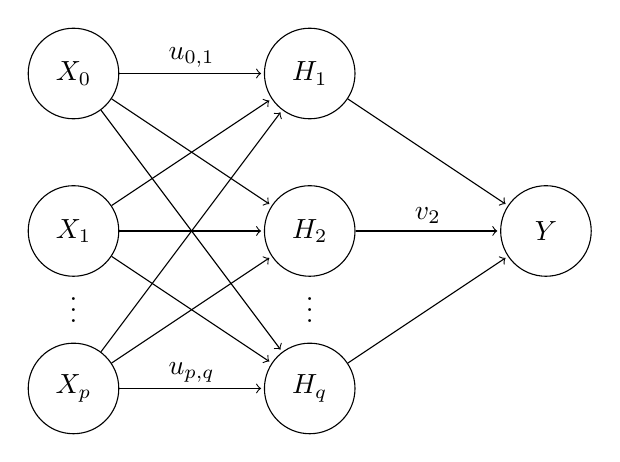
\begin{tikzpicture}[shorten >=1pt]
        \tikzstyle{unit}=[draw,shape=circle,minimum size=1.15cm]

        \node[unit](x0) at (0,4){$X_0$};
        \node at (1.5,4.2){$u_{0,1}$};
        \node[unit](x1) at (0,2){$X_1$};
        \node(dots) at (0,1.1){\vdots};
        \node[unit](xp) at (0,0){$X_p$};
        \node at (1.5,0.2){$u_{p,q}$};

        \node[unit](h1) at (3,4){$H_1$};
        \node[unit](h2) at (3,2){$H_2$};
        \node at (4.5,2.2){$v_{2}$};
        \node(dots) at (3,1.1){\vdots};
        \node[unit](hq) at (3,0){$H_q$};
        
        \node[unit](y) at (6,2){$Y$};
 
        \draw[->] (x0) -- (h1);
        \draw[->] (x0) -- (h2);
        \draw[->] (x0) -- (hq);

        \draw[->] (x1) -- (h1);
        \draw[->] (x1) -- (h2);
        \draw[->] (x1) -- (hq);

        \draw[->] (xp) -- (h1);
        \draw[->] (xp) -- (h2);
        \draw[->] (xp) -- (hq);
        
        \draw[->] (h1) -- (y);
        \draw[->] (h2) -- (y);
        \draw[->] (hq) -- (y);

    \end{tikzpicture}
\end{center}
%---------------TikZ_______________

\noindent Een opeenstapeling van lineaire transformaties blijft een lineaire transformatie. Om uit het lineaire regime te ontsnappen moeten we een niet-lineaire transformatie op iedere laag toepassen, de zogenoemde activatiefunctie.

\subsection{Logistische neurale netwerken (sigmoid)}
De sigmoid-activatiefunctie zal toegepast worden, waardoor de volgende formule en netwerk ontstaan:
\[Y=\sum\limits_{j=1}^qv_j\varphi(\sum\limits_{i=0}^pu_{ij}X_i)=(\textbf{U}\overrightarrow{v}) \overrightarrow{X}=\overrightarrow{\beta} \overrightarrow{X}\]

\begin{center}
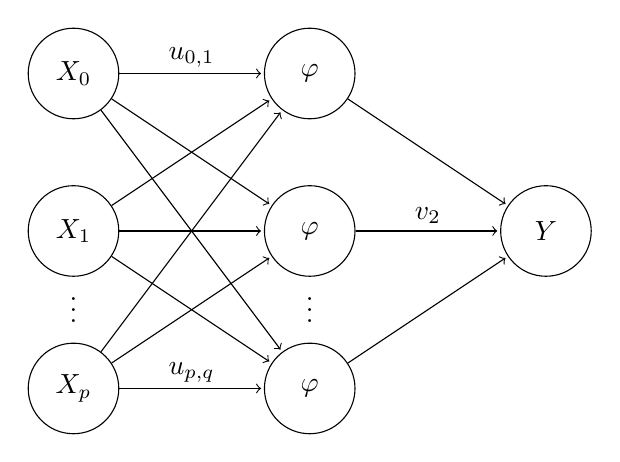
\begin{tikzpicture}[shorten >=1pt]
        \tikzstyle{unit}=[draw,shape=circle,minimum size=1.15cm]

        \node[unit](x0) at (0,4){$X_0$};
        \node at (1.5,4.2){$u_{0,1}$};
        \node[unit](x1) at (0,2){$X_1$};
        \node(dots) at (0,1.1){\vdots};
        \node[unit](xp) at (0,0){$X_p$};
        \node at (1.5,0.2){$u_{p,q}$};

        \node[unit](h1) at (3,4){$\varphi$};
        \node[unit](h2) at (3,2){$\varphi$};
        \node at (4.5,2.2){$v_{2}$};
        \node(dots) at (3,1.1){\vdots};
        \node[unit](hq) at (3,0){$\varphi$};
        
        \node[unit](y) at (6,2){$Y$};
 
        \draw[->] (x0) -- (h1);
        \draw[->] (x0) -- (h2);
        \draw[->] (x0) -- (hq);

        \draw[->] (x1) -- (h1);
        \draw[->] (x1) -- (h2);
        \draw[->] (x1) -- (hq);

        \draw[->] (xp) -- (h1);
        \draw[->] (xp) -- (h2);
        \draw[->] (xp) -- (hq);
        
        \draw[->] (h1) -- (y);
        \draw[->] (h2) -- (y);
        \draw[->] (hq) -- (y);

    \end{tikzpicture}
\end{center}

\noindent De structuur van het feed forward netwerk is:\\
\begin{minipage}{0.6\textwidth}
\begin{enumerate}
    \item Invloer \hfill $\overrightarrow{X}$
    \item Matrix vermenigvuldiging (weights) \hfill $\textbf{U}\overrightarrow{X}$
    \item niet-lin. transformatie (activatie) \hfill $\varphi (\textbf{U}\overrightarrow{X})$
    \item lin. combinatie \hfill $\overrightarrow{v}\varphi (\textbf{U}\overrightarrow{X})$
\end{enumerate}
\end{minipage}

\noindent Er kunnen ook meerdere lagen toegevoegd worden. Het is niet per definitie zo dat meer lagen voor een beter resultaat zorgen. Het aantal nodes is minstens net zo belangrijk. Voor meer informatie, zie \textit{Deep, Skinny Neural Networks are not Universal Approximators}.\\

\noindent
Twee nodes per laag kan mogelijk geen goede voorspelling maken, want er zitten maar twee grensvlakken aan verbonden als er maar twee nodes per layer aanwezig zijn. Zo kan er bijvoorbeeld geen cirkel gevormd worden bij 6, 2-dimensionale layers (a), terwijl dat met een enkele 3-node-layer wel gaat (b).
\begin{figure}[h]
    \centering
    \includegraphics[width=0.8\linewidth]{Images/layers probleem.png}
    \caption*{}
    \label{fig:layer}
\end{figure}\vspace{-1cm}

\subsection{Hoe trainen we een neuraal netwerk?}
Neem een netwerk met $l$ lagen, van groottes $n_1$ t/m $n_l$, activatiefunctie $\varphi^1$ t/m $\varphi^l$ en gewichten $\textbf{U}^1$ t/m $\textbf{U}^l$. Dus:
\[Y=g(\overrightarrow{X})=\varphi^l(\textbf{U}^l\varphi^{l-1}(\textbf{U}^{l-1}\dots\varphi^2(\textbf{U}^2\varphi(\textbf{U}\overrightarrow{X}))))\]
We introduceren een loss functie $L(\hat{y}),y$. 
\[L(\hat{y}),y=L(g(\overrightarrow{x}),y)\]

\noindent Het gewicht $u_{ij}^k$ is het gewicht dat hoort bij de pijl van de node $i$ in laag $k-1$ naar node $j$ in laag $k$. We kunnen met de kettingregel de loss differentiëren naar $u_{ij}^k$.
\[\frac{\partial L}{\partial u_{ij}^k}=L'\varphi^{l'}\textbf{U}^l\varphi^{l-1'}\dots \varphi^{k+1'}\textbf{U}^{k+1}\varphi_i^{k-1}\]
waar $\varphi_i^{k-1}$ de activatie van de $i^{de}$ neuron in laag $k-1$ is.\\

\noindent We zien dat de afgeleide alleen afhangt van:
\begin{itemize}
    \item de afgeleiden van de lagen rechts
    \item de activatie van de laag links
\end{itemize}
We kunnen dus redelijk efficiënt al deze afgeleiden van rechts naar links uitrekenen. Dit algoritme heet \textit{back propagation}. Dit wordt gebruikt in het volgende neurale netwerk cyclus:
\begin{enumerate}
    \item Bepalen van gewichten
    \item De loss functie bepalen met de feedforward fase
    \item Back propagation vanaf loss functie om gewichten te optimaliseren
    \item Repeat
\end{enumerate}

\subsection{Stochastic Gradient Descent}
\noindent Om onze gemiddelde loss $\bar{L}$ nu te minimaliseren gaan we als volgt te werk:
\begin{enumerate}
    \item We splitsen de data op in kleine random batches
    \item Voor iedere waarneming in een batch bepalen we $\frac{\partial L}{\partial u_{ij}^k}$
    \item Deze afgeleiden middelen we tot $\frac{\partial \bar{L}}{\partial u_{ij}^k}$
    \item We passen de gewichten als volgt aan:
    \[u_{ij}^k(t+1)=u_{ij}^k(t)-r\frac{\partial \bar{L}}{\partial u_{ij}^k}\]
    hier is $r$ de \textit{learning rate}.
    \item Als de volledige dataset op deze manier is doorlopen noemen we dit een epoch en herhalen we dit proces.
\end{enumerate}

\textbf{Batchsize}\\
Een te kleine batchsize kan zorgen voor slecht trainen van het model, omdat er dan van enkele klassen data in een batch kan zitten. Als het model enkel daarop traint, traint het niet op alle klassen (traint te specifiek). Een batchsize van 32 is meestal groot genoeg, representatief voor data. Bij veel klassen kies je voor een grotere batchsize. 

\subsection{Vanishing Gradient Problem}
\noindent Veel activatiefuncties vlakken af bij grote waardes van hun invoer. Hun afgeleides zijn dus heel klein en worden ook nog met elkaar vermenigvuldigd. Het gevolg is dat $u_{ij}^k$ voor kleine k nauwelijks aangepast word en dat het netwerk nauwelijks leert. Om dat probleem (deels) op te lossen wordt tegenwoordig vaak de ReLU-activatiefunctie gebruikt.
\begin{figure}[h]
    \centering
    \includegraphics[width=0.6\linewidth]{Images/vgp.png}
    \caption*{}
    \label{fig:layer}
\end{figure}

\newpage
\subsection{Voorbereiding}
Voorbereiding van het maken van een neuraal netwerk:
\begin{itemize}
    \item Probleemanalyse
    \item Data verzameling
    \item Train/test split
    \item Data verkenning
    \item Keuze loss-functie
    \item Keuze metrieken
\end{itemize}
\textbf{Feature selection}\\
Model kan slechter scoren als er betekenisloze variabelen in het model verwerkt zijn. Je wilt de variabelen afgaan en analyseren welke belangrijk zijn.\\

\textbf{Problemen met modelverbetering}
\begin{table}[h]
    \centering
    \begin{tabular}{|p{6cm}|p{5cm}|}
    \hline
    \textbf{Probleem} & \textbf{Oplossing}\\ \hline
         Trainen doet niks, je loss veranderd niet of nauwelijks per epoch en het model leert niks. & Learning rate of batchsize aanpassen. \\ \hline
         Het model traint wel, maar krijgt geen goede resultaten. Het verslaat simpele baselines niet of nauwelijks. Denk aan val\_acc die niet omhoog gaat. & Data probleem/model: (1) te weinig data, (2) misclassificatie, (3) verkeerde aanpak.\\\hline
         Het model traint en krijgt redelijke resultaten, maar na verloop van tijd gaat het nooit overfitten en blijft het dus underfit. Denk aan stagneren van train\_acc en val\_acc. & Meer lagen toevoegen/lagen groter maken.\\ \hline
         Duurt lang. & Geduld hebben. \\ \hline
    \end{tabular}
    \caption*{}
    \label{tab:my_label}
\end{table}

%plaatjes toevoegen

\textbf{Regularisatie}\\
Na het behalen van een goede loss-epoch-grafiek willen we het moment van overfitten zo lang mogelijk uitstellen. 
\begin{itemize}
    \item Early stopping (stoppen bij laagste val\_acc)
    \item Netwerk verkleinen als groot netwerk overfit, te klein blijft underfit. Probeer de juiste samenstelling te vinden)
    \item $L_1$ en/of $L_2$ regularisatie. (bij grote modellen werkt het niet goed)
    \item Dropout (willekeurige activaties op 0 zetten, bij grotere modellen werkt het wel goed)
\end{itemize}
\begin{figure}[h]
    \centering
    \includegraphics[width=0.8\linewidth]{Images/regularisaties.png}
    \caption*{}
    \label{fig:regularisatie}
\end{figure}
\begin{figure}[h!]
    \centering
    \includegraphics[width=0.8\linewidth]{Images/samenvattingNN.png}
    \caption*{}
    \label{fig:samenvatting}
\end{figure}
}

\newpage
\
\newpage
{\large
\textbf{{\LARGE Week 9}}
\subsection{Convolutionele Neurale Netwerken}
Beeldherkenningstaken:
\begin{itemize}
    \item Single-label classificatie
    \item Multi-label classificatie (meerdere dingen tegelijk herkennen)
    \item Segmentatie (classificatie op pixelniveau)
    \begin{itemize}
        \item Semantic
        \item Instance
    \end{itemize}
    \item Object Detection
\end{itemize}

\textbf{Waarom dense layers niet werken bij beeldmateriaal}
\begin{itemize}
    \item Globaliteit -- iedere mogelijke combinatie van inputs zou een mogelijk signaal kunnen bevatten.
    \item Deze signalen verschillen allemaal van elkaar.
\end{itemize}
Voor beeldmateriaal gelden de volgende aannames:
\begin{itemize}
    \item Lokaliteit -- Alleen combinaties van inputs met zijn buren bevatten zinvolle signalen.
    \item Translatie-invariantie -- Deze signalen blijven hetzelfde als de input met de buren verplaatst.
\end{itemize}
Een convolutielaag is een dense layer waar merendeel van de gewichten uit zijn gezet. \textit{padding = 'same'} plaatst virtuele waarden aan rand die dezelfde waardes hebben als de pixels ernaast.

\noindent Een aantal instellingen kunnen verder het aantal gewichten beïnvloeden:
\begin{itemize}
    \item Kernel size
    \item Padding (vooral bij segmentatie, je wilt daar grootte behouden)
    \item Stride (stapgrootte kernel size)
    \item Pooling (max, global average, low pooling van de filtercombinatie)
\end{itemize}
Max pooling werkt beter dan het nemen van strides, maar verliest hiermee wel informatie over waar deze features zich bevinden (belangrijk voor segmentatie)\\

\subsubsection{Typische architectuur}
\begin{itemize}
    \item Data augmentatie
    \item Meerdere convolutie blokken
    \begin{itemize}
        \item Een of meer convolutielagen
        \item Max pooling om het aantal gewichten laag te houden
    \end{itemize}
    \item Flatten
    \item Een dense layer voor de uitvoer
\end{itemize}
\subsubsection{Transfer Learning}
De enorme voorgetrainde netwerken kunnen redelijk algemene patronen herkennen die toepasbaar zijn op heel veel andere beeldtaken. Daarom kan het bij weinig data handig zijn om een model te pakken die bijvoorbeeld een ImageNet-competitie heeft gewonnen. Pak de convolutielagen van deze netwerken en vervang de dense layer en loss-functie. \\

Werkwijze:
\begin{enumerate}
    \item Voeg eigen dense layer toe aan voorgetrainde basis
    \item Bevries gewichten van voorgetrainde basis
    \item Train je netwerk
    \item Finetunen
    \item Ontvries gewichten met de laatste lagen (met factor 10 lagere learning rate)
    \item Opnieuw trainen
\end{enumerate}

\subsubsection{Transpose Convolutie}
\begin{itemize}
    \item Onze invoer bestaat uit $200\times 200$ pixel plaatjes.
    \item We willen deze plaatjes segmenteren, ofwel we kennen een klasse toe aan iedere pixel
    \item Onze uitvoer moet dus bestaan uit $200\times 200$ geclassificeerde pixels
\end{itemize}
Echter:
\begin{itemize}
    \item We nemen convoluties met een stride van 2
    \item Dus na deze convolutie halveert onze resolutie
    \item Uiteindelijk hebben we een $25 \times 25$ 'plaatje' met 256 features
\end{itemize}
Een transpose convolutie probeert te leren hoe deze convoluties weer ongedaan gemaakt moeten worden. De (200,200,\textbf{3}) van de invoer geeft het aantal kleurenchannels weer (RGB), terwijl de (200,200,\textbf{3}) van de uitvoer het aantal klasses weergeeft.

\subsubsection{$1\times 1$ convoluties}
Pixels worden halveert, aantal filters/features verdubbelen. Kan tot een convolutielaag met 1 pixel en heel veel filters. Deze convoluties worden soms gebruikt om het aantal features te veranderen zonder ruimtelijke informatie te veranderen. Ze zijn een voorbeeld van een Network-in-network laag.
\begin{figure}[h!]
    \centering
    \includegraphics[width=0.4\linewidth]{Images/convfilters.png}
    \caption{$1\times 1$ convoluties}
    \label{fig:filters}
\end{figure}

\subsubsection{Residual connecties}
Pixels worden halveert, aantal filters/features verdubbelen. Dan ontstaan er hele diepe netwerken. Kan niet notatie 'model.add()' gebruiken, want lopen 2 dingen parallel aan elkaar. Doen zodat het nog goed blijft trainen.

\begin{figure}[h!]
    \centering
    \includegraphics[width=0.5\linewidth]{Images/residualnetsdepth.png}
    \caption{Residual netwerk}
    \label{fig:filters}
\end{figure}

\noindent Het idee van residual connections is om de (gradient van de) fout dieper in het netwerk te laten propageren, zodat ook diepere lagen kunnen trainen. Dit doen we door de activatie van de diepere lagen bij nieuwe lagen op te tellen.

\begin{figure}[h!]
    \centering
    \includegraphics[width=0.25\linewidth]{Images/residuals.png}
    \caption{Residual connectie}
    \label{fig:filters}
\end{figure}
\begin{itemize}
    \item De residual bevat een $1\times 1$ convolutie zonder activatie om te zorgen dat het aantal filters hetzelfde is als de uitvoer van het overgeslagen convolutieblok.
    \item Convoluties in het convolutieblok moeten met padding werken om te zorgen dat de resolutie niet veranderd.
    \item Als het convolutieblok gebruik maakt van pooling zal deze $1\times 1$ convolutie met strides moeten werken zodat de resolutie hetzelfde blijft.
    \item Aan het eind wordt de residual connection bij de uitvoer van het convolutieblok opgeteld.
\end{itemize}

\begin{figure}[h!]
    \centering
    \includegraphics[width=0.8\linewidth]{Images/residualnetwork.png}
    \caption{Code van een simpel residual netwerk}
    \label{fig:filters}
\end{figure}
\newpage
\subsubsection{Global Average Pooling}
Convolutielaag (in plaats van dense en flatten layer) die evenveel filters als klasses heeft. Iedere filter komt overeen met iets dat je wilt herkennen. Gemiddelde van alle filters in de convolutielaag is de klasse die eruit komt. 

\noindent Bij global average pooling wordt het gemiddelde van de hele filter genomen. De laatste convolutionele laag heeft even veel filters als er te voorspellen klassen zijn. Deze filters worden over de hele laag gemiddeld. \href{https://arxiv.org/pdf/1312.4400.pdf}{Bron}

\begin{figure}[h!]
    \centering
    \includegraphics[width=0.5\linewidth]{Images/gap.png}
    \caption{global average pooling}
    \label{fig:filters}
\end{figure}

\subsubsection{Batch Normalisation}
Batch normalisatie wordt gebruikt om het aantal parameters te verkleinen. De uitvoer van een convolutionele laag wordt voor de activatiefunctie genormaliseerd.
\begin{itemize}
    \item Gemiddelde 0
    \item Variantie 1
\end{itemize}
Omdat de activatiefunctie het stekt veranderd bij nul per filter, is er nu geen bias nodig in de convolutionele laag.
\begin{figure}[h!]
    \centering
    \includegraphics[width=0.6\linewidth]{Images/batchnorm.png}
    \caption{Batch normalisatie}
    \label{fig:filters}
\end{figure}

\subsubsection{Separabele convoluties}
In een gewone convolutielaag worden alle filters samen genomen, wat voor veel parameters zorgt. Dus splitsen we de filters en pas je toe op de diepere lagen (niet kleuren maar kleine randjes).
\begin{figure}[h!]
    \centering
    \includegraphics[width=0.6\linewidth]{Images/batchnorm1.png}
    \caption{Separabele convoluties}
    \label{fig:filters}
\end{figure}

\subsubsection{Interpreteerbaarheid}
In het algemeen word gezegd dat neurale netwerken black boxes zijn, het is niet echt duidelijk hoe ze tot hun voorspellingen komen. Echter, omdat CNN's visuele informatie verwerken is het hier mogelijk om toch redelijk veel inzicht te krijgen in hoe het model werkt.
\begin{itemize}
    \item Je kan de activatie van je filters plotten
    \item Je kan achterhalen op welk patroon een filter maximaal reageert
    \item Je kan achterhalen welke pixels in een afbeelding de sterkste invloed op de voorspelling hadden
\end{itemize}

\subsubsection{Gebruik pretrained model}
\begin{figure}[h!]
    \centering
    \includegraphics[width=0.9\linewidth]{Images/xception.png}
    \caption{Xception aanroepen}
    \label{fig:filters}
\end{figure}


}

\end{document}
